%%%%%%%%%%%%%%%%%%%%%%%%%%%%%%%%%%%%%%%%%%%%%%%%%%%%%%%%%%%%%%%%%%%%%%%%%%%%%%%%%%%%%%%%%%%%%%%%%%%%%%%%%%
%Write by:ShuwenHe
%Date:20230613
%%%%%%%%%%%%%%%%%%%%%%%%%%%%%%%%%%%%%%%%%%%%%%%%%%%%%%%%%%%%%%%%%%%%%%%%%%%%%%%%%%%%%%%%%%%%%%%%%%%%%%%%%%

%%%%%%%%%%%%%%%%%%%%%%%%%%%%%%%%%%%%%%%%%%%%%%%%%%%%%%%%%%%%%%%%%%%%%%%%%%%%%%%%%%%%%%%%%%%%%%%%%%%%%%%%%%
\documentclass[12pt,twiside,a4paper]{ctexbook}
\usepackage[centertags]{amsmath}
\usepackage{amsfonts}
\usepackage{amsthm}
\usepackage{newlfont}
\usepackage{makeidx}
\usepackage{wasysym}
\usepackage{geometry} 
\usepackage{graphics}
\usepackage{slashbox} 
\usepackage{fancyhdr} 
\usepackage[pdftex]{graphicx}
\usepackage{epstopdf}
\usepackage{cite}
\usepackage{listings}
\usepackage{tocbibind}
\usepackage[numbers,sort&compress]{natbib}

\setlength\parskip{\baselineskip}
\setcounter{tocdepth}{8} % 生成目录层级
\setcounter{secnumdepth}{4}
\renewcommand\thesection{\arabic{section}}
\usepackage[pdfstartview=FitH,CJKbookmarks=true,bookmarks,bookmarksnumbered=true,
    colorlinks=true,citecolor=black,linkcolor=black,anchorcolor=green,urlcolor=black]{hyperref}
\usepackage{titlesec}
\usepackage{tabularx}
\titleformat{\chapter}[display]{\normalfont\huge\bfseries\center}{\chaptertitlename}{1pt}{\Huge}
\titleformat{\section}{\normalfont\Large\bfseries}{\thesection}{1em}{}
\titleformat{\subsection}{\normalfont\large\bfseries}{\thesubsection}{1em}{}
\titleformat{\subsubsection}{\normalfont\normalsize\bfseries}{\thesubsubsection}{1em}{}
\titleformat{\paragraph}[runin]{\normalfont\normalsize\bfseries}{\theparagraph}{1em}{}
\titleformat{\subparagraph}[runin]{\normalfont\normalsize\bfseries}{\thesubparagraph}{1em}{}
\titlespacing*{\chapter} {0pt}{10pt}{10pt}
\titlespacing*{\section} {0pt}{0.5ex plus 1ex minus .2ex}{0.3ex plus .2ex}
\titlespacing*{\subsection} {0pt}{0.25ex plus 1ex minus .1ex}{0.5ex plus .1ex}
\titlespacing*{\subsubsection}{0pt}{3.25ex plus 1ex minus .2ex}{1.5ex plus .2ex}
\titlespacing*{\paragraph} {0pt}{3.25ex plus 1ex minus .2ex}{1em}
\titlespacing*{\subparagraph} {\parindent}{3.25ex plus 1ex minus .2ex}{1em}
\numberwithin{chapter}{part}
\geometry{left=2.0cm,right=20mm,top=25mm,bottom=25mm}
\let\cleardoublepage\clearpage
%%%%%%%%%%%%%%%%%%%%%%%%%%%%%%%%%%%%%%%%%%%%%%%%%%%%%%%%%%%%%%%%%%%%%%%%%%%%%%%%%%%%%%%%%%%%%%%%%%%%%%%%%%

%%%%%%%%%%%%%%%%%%%%%%%%%%%%%%%%%%%%%%%%%%%%%%%%%%%%%%%%%%%%%%%%%%%%%%%%%%%%%%%%%%%%%%%%%%%%%%%%%%%%%%%%%%
%mathematics
\usepackage{amssymb}
\usepackage{diagbox}
%%%%%%%%%%%%%%%%%%%%%%%%%%%%%%%%%%%%%%%%%%%%%%%%%%%%%%%%%%%%%%%%%%%%%%%%%%%%%%%%%%%%%%%%%%%%%%%%%%%%%%%%%%

%%%%%%%%%%%%%%%%%%%%%%%%%%%%%%%%%%%%%%%%%%%%%%%%%%%%%%%%%%%%%%%%%%%%%%%%%%%%%%%%%%%%%%%%%%%%%%%%%%%%%%%%%%
%
%%%%%%%%%%%%%%%%%%%%%%%%%%%%%%%%%%%%%%%%%%%%%%%%%%%%%%%%%%%%%%%%%%%%%%%%%%%%%%%%%%%%%%%%%%%%%%%%%%%%%%%%%%

%%%%%%%%%%%%%%%%%%%%%%%%%%%%%%%%%%%%%%%%%%%%%%%%%%%%%%%%%%%%%%%%%%%%%%%%%%%%%%%%%%%%%%%%%%%%%%%%%%%%%%%%%%
%
\usepackage{tipa} % 音标
%%%%%%%%%%%%%%%%%%%%%%%%%%%%%%%%%%%%%%%%%%%%%%%%%%%%%%%%%%%%%%%%%%%%%%%%%%%%%%%%%%%%%%%%%%%%%%%%%%%%%%%%%%

%%%%%%%%%%%%%%%%%%%%%%%%%%%%%%%%%%%%%%%%%%%%%%%%%%%%%%%%%%%%%%%%%%%%%%%%%%%%%%%%%%%%%%%%%%%%%%%%%%%%%%%%%%
\begin{document}
%%%%%%%%%%%%%%%%%%%%%%%%%%%%%%%%%%%%%%%%%%%%%%%%%%%%%%%%%%%%%%%%%%%%%%%%%%%%%%%%%%%%%%%%%%%%%%%%%%%%%%%%%%

\author
{
%Peking University\\
%北京大学\\
%ShuwenHe\\
%何书文\\
%1201220707@pku.edu.cn
Richard He \& Ritchie He
}

%%%%%%%%%%%%%%%%%%%%%%%%%%%%%%%%%%%%%%%%%%%%%%%%%%%%%%%%%%%%%%%%%%%%%%%%%%%%%%%%%%%%%%%%%%%%%%%%%%%%%%%%%%
%\centerline{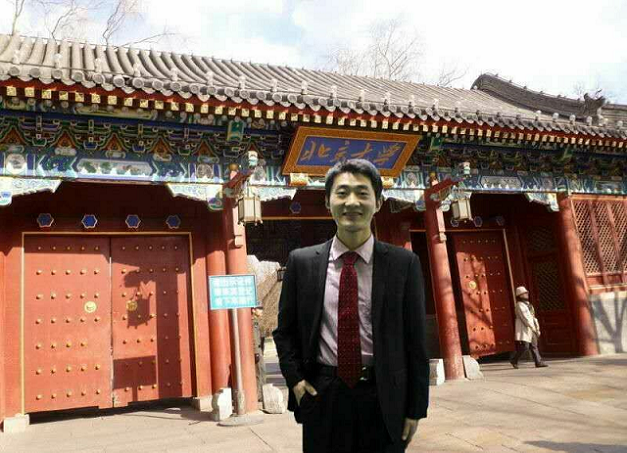
\includegraphics{shuwenhe.png}}
%写好一本书:工匠精神!用心打造!夜深写于北京大学图书馆。作者亲自一线带课,所带学生多人保送或考入清华北大,根据多年清华附中、101中学、人大附中、北大附中、十一学校,考试真题分析经验所得。用此书考上心目中名校学生无数!何书文北京大学硕士,资深数学名师、信息学竞赛算法名师,所带学生多名考入人大附中早培、清华附中优才、101 实验班、北大附中实验班等名校。全国中学数学联赛、全国中学数学竞赛的辅导老师,全国NOI、CSP信息学竞赛辅导名师。何书文老师在北京大学学习期间立志从事教育事业,帮学生授业解惑。何书文老师小学期间学习奥数,并多次获奖,为以后的学习与研究打下良好基础。何书文 老师在中学阶段数学、物理均获奖。何书文老师在小学中学期间一直为数学课代表,中小学大学期间担任班长,何书文老师在北京大学被选为科技一苑苑长,组织北大同学积极参与校各项活动,积极参与校学生会工作,何书文老师被北京大学评为优秀入党积极分子.何书文老师经常参加北京大学数学课题的研讨班。何书文 老师是北京大学数学系暑期学校全国选出40 名优秀中青年数学人才之一,参加伦敦国王学院、美国杜克大学、美国纽约大学、加拿大多伦多大学教授组成的学术研讨班,研究PDE(偏微分方程),量子力学方面的数学课题的研究工作,并获得优异成绩结业。何书文老师作为项目经理用数学建模方法给大型企业开发软件,用数学方法规划提高企业产能协作效率。何书文 老师致力于数学方面的教学与研究工作,所带多名孩子已经被点优才进入清华附中创新班,101 实验班,人大附中早培班,是家长值得信赖的老师。考上学生继续跟随何书文老师学习全国数学联赛,全国数学竞赛系列课程,同时学习NOI、IOI、ACM算法编程竞赛。
%%%%%%%%%%%%%%%%%%%%%%%%%%%%%%%%%%%%%%%%%%%%%%%%%%%%%%%%%%%%%%%%%%%%%%%%%%%%%%%%%%%%%%%%%%%%%%%%%%%%%%%%%%

%%%%%%%%%%%%%%%%%%%%%%%%%%%%%%%%%%%%%%%%%%%%%%%%%%%%%%%%%%%%%%%%%%%%%%%%%%%%%%%%%%%%%%%%%%%%%%%%%%%%%%%%%%
\title{English英语}
\maketitle
\tableofcontents % 显示目录
\newpage
\pagestyle{fancy}
%%%%%%%%%%%%%%%%%%%%%%%%%%%%%%%%%%%%%%%%%%%%%%%%%%%%%%%%%%%%%%%%%%%%%%%%%%%%%%%%%%%%%%%%%%%%%%%%%%%%%%%%%%

%\lhead{
\includegraphics{shuwenedu.png}}
%\rhead{科技特长生升学规划 何校长 电话微信15010729356}
%\lfoot{
\includegraphics{pku.png}算法第一人北大何书文}
%\rfoot{改变您家孩子命运的老师}
%%%%%%%%%%%%%%%%%%%%%%%%%%%%%%%%%%%%%%%%%%%%%%%%%%%%%%%%%%%%%%%%%%%%%%%%%%%%%%%%%%%%%%%%%%%%%%%%%%%%%%%%%%

%%%%%%%%%%%%%%%%%%%%%%%%%%%%%%%%%%%%%%%%%%%%%%%%%%%%%%%%%%%%%%%%%%%%%%%%%%%%%%%%%%%%%%%%%%%%%%%%%%%%%%%%%%
\begin{center}

\chapter{pronunciation发音}
\section{latex}
\begin{tabularx}{\textwidth}{|c|X|}
\hline
\textbf{英语音标} & \textbf{LaTeX音标} \\
\hline
\textipa{I} & \verb|\textipa{I}| \\
e & \verb|\textipa{e}| \\
\textipa{\textepsilon} & \verb|\textipa{\textepsilon}| \\
\textipa{A}& \verb|\textipa{A}| \\
\textipa{o} & \verb|\textipa{o}| \\
\textipa{U} & \verb|\textipa{U}| \\
u & \verb|\textipa{u}| \\
ə & \verb|\textipa{@}| \\
\textipa{g} & \verb|\textipa{g}| \\
\textipa{T} & \verb|\textipa{T}| \\
ð & \verb|\textipa{D}| \\
\textipa{S} & \verb|\textipa{S}| \\
\textipa{Z} & \verb|\textipa{Z}| \\
ŋ & \verb|\textipa{N}| \\
\textturnscripta & \verb|\textipa{\textturnscripta}|\\
\textipa{\textopeno} & \verb|\textipa{\textopeno}|\\
\textprimstress & \verb|\textprimstress|\\
\textipa{\textlengthmark} & \verb|\textlengthmark|\\
\hline
\end{tabularx}
\end{center}
\section{48个国际音标}
\subsection{前元音\textipa{I}}
\begin{tabular}{|c|c|c|}
\hline
音标 & 词汇 & 译意 \\
\hline
/k\textipa{I}t/ & kit & n. 成套工具 \\
/b\textipa{I}d/ & bid & n. 投标 \\
/h\textipa{I}m/ & hymn & n. 圣歌 \\
/ˈ\textprimstress m\textipa{I}n\textipa{I}t/ & minute & n. 分钟;会议记录 \\

\hline
\end{tabular}

\subsection{前元音\textipa{I}\textlengthmark}
\subsection{3}
\subsection{4}
\subsection{5}
\subsection{6}
\subsection{7}
\subsection{8}
\subsection{9}
\subsection{10}
\subsection{11}
\subsection{12}
\subsection{13}
\subsection{14}
\subsection{15}
\subsection{16}
\subsection{17}
\subsection{18}
\subsection{19}
\subsection{20}
\subsection{21}
\subsection{22}
\subsection{23}
\subsection{24}
\subsection{25}
\subsection{26}
\subsection{27}
\subsection{28}
\subsection{29}
\subsection{30}
\subsection{31}
\subsection{32}
\subsection{33}
\subsection{34}
\subsection{35}
\subsection{36}
\subsection{37}
\subsection{38}
\subsection{39}
\subsection{40}
\subsection{41}
\subsection{42}
\subsection{43}
\subsection{44}
\subsection{45}
\subsection{46}
\subsection{47}
\subsection{48}
\chapter{Vocabulary词汇}
\section{a}
/\textprimstress æl\textipa{g}ər\textipa{I}ðəm/\\
algorithm\\
算法

\section{b}
/bre\textipa{I}s/\\
brace\\

\section{c}
\section{d}
\section{e}
/\textprimstress el\textipa{I}mənt/\\
element\\
元素

\section{f}
\section{g}
\section{h}
\section{i}
/\textprimstress\textipa{I}ŋkrəmənt/\\
increment\\
自增\\
词根词缀: in- 入 , 向内 + -cre- 生长 + -ment 名词词尾

\section{j}
\section{k}
\section{l}
\section{m}
/ˌmæθəˈmætɪks/\\0
mathematics
3.1415926..。。
/\textprimstress m\textturnscripta d\textipa{I}fa\textipa{I}/\\
modify\\
v. 修改\\
词根词缀: -mod- 量器 + -i- + -fy 动词词尾

\section{n}
\section{o}
/\textprimstress\textipa{\textopeno}\textipa{\textlengthmark}r\textipa{I}d\textipa{Z}\textipa{I}n/\\
origin\\
n. 起源

/əˈrɪdʒən(ə)l/\\
original

\section{p}
\section{q}
\section{r}
/\textprimstress refrəns/\\
reference\\
引用\\
词根词缀: re- 回 + -fer- 拿取 + -ence 名词词尾

\section{s}
\section{t}
/temp/\\
temp\\
临时变量
\section{u}
\section{v}
/\textprimstress vektər/\\
vector\\
向量
\section{w}
\section{x}
\section{y}
\section{z}

\chapter{world-famous masterpiece世界名著}
\section{New Concept新概念}
\subsection{第一册}
\subsection{第二册}
\subsection{第三册}
\subsection{第四册}
\section{The Old Man and the Sea}
\section{chapter1}

\clearpage
\end{document}
